\documentclass{ltjsarticle}

\usepackage{luatexja}
\usepackage{graphicx}
\usepackage[colorlinks=true,linkcolor=blue,citecolor=blue,urlcolor=blue]{hyperref}
\usepackage{xcolor}
\usepackage{mathtools}
\usepackage{siunitx}
\usepackage{amsmath}
\usepackage{amssymb}
\usepackage{sepnum} % sepnumパッケージを読み込む
\usepackage{at}
\usepackage{bm}
\usepackage{cancel}
\usepackage{float} % ← プリアンブルに追加
\usepackage{titlesec}
\numberwithin{equation}{section} % 数式番号をセクションごとに分ける
\titleformat{\subsubsection}
  {\normalfont\large\bfseries}
  {\thesubsubsection}{1em}{}

\newcommand{\underlab}[3][.35ex]{%
  \mathrel{\mathop{#2}\limits_{\mathclap{\lower#1\hbox{\text{\footnotesize\textcircled{\scriptsize #3}}}}}}%
}

\newcommand{\ctext}[1]{\raise0.2ex\hbox{\textcircled{\scriptsize{#1}}}}

\usepackage[normalem]{ulem} % \uline, \uwave

% 直線 → \ulineunder、波線 → \uwaveunder
\newcommand{\ulineunder}[2]{%
  \underset{\smash{\text{\scriptsize #2}}}{\uline{\ensuremath{#1}}}%
}
\newcommand{\uwaveunder}[2]{%
  \underset{\smash{\text{\scriptsize #2}}}{\uwave{\ensuremath{#1}}}%
}

% 下線の“下げ量”と太さ（グローバル設定）
\setlength{\ULdepth}{1.2ex} 
\renewcommand\ULthickness{0.8pt} % 波線/直線の太さ


\usepackage[most]{tcolorbox}
\newtcolorbox{eqbox}[1]{%
  enhanced,
  colback=white, colframe=black,
  boxrule=0.4pt, arc=6pt,
  left=8pt, right=8pt, top=8pt, bottom=8pt, % 余白
  title={#1},                 % ← 引数がタイトルになる
  fonttitle=\bfseries,        % タイトルの体裁
  coltitle=black,
  colbacktitle=gray!10,       % タイトル帯の背景色（要らなければ white）
  attach boxed title to top left={yshift=-2mm, xshift=6pt}, % 箱内の左上に配置
  boxed title style={sharp corners, boxrule=0pt}, % タイトル枠線なし
}


\title{Introduction to Plasma Physics}
\author{中 陽太}
\date{2026年2月21日}

\begin{document}

\maketitle

% 目次
\tableofcontents

\section*{前書き}
 以下の内容は、主に

\cite{a} Francis F. Chen, "Introduction to Plasma Physics and Controlled Fusion"\par
\cite{b} 宮本健郎 『プラズマ物理の基礎』\par
\cite{c} EMANの物理学\\
を参照している。



\section{拡散と抵抗} \label{section5}
\subsection{弱電離気体中の拡散と易動度} \label{section5.1}
前章で平衡条件を求めるときに仮定した，無限で均一なプラズマは，当然ながら極めて理想化されたものである．現実的なプラズマには密度勾配が存在し，プラズマは低密度領域へ拡散する傾向がある．
制御核融合反応における中心的な課題は，磁場を用いてこの拡散を抑制することである．しかしここではまず，磁場問題に取り組む前に，磁場が存在しない場合の拡散を考える．
荷電粒子が互いに衝突するよりも，主として中性原子と衝突するような弱電離プラズマと仮定すれば，さらに単純化できる．完全電離プラズマの場合は，非線形方程式となり，簡単な解析解がほとんど存在しないので，後節に譲る．

ここでは，高密度の中性原子を背景とした非一様なイオンや電子の分布を考える．プラズマが圧力勾配や電場による力によって拡散するにつれ，個々の粒子はランダムウォークを経験し，
中性原子と頻繁に衝突する．まず，原子論からの定義について簡単に振り返ることから始める．

\subsubsection{衝突パラメータ} \label{section5.1.1}
電子が中性原子と衝突すると，反射する角度によって，初期の運動量の何パーセントかを失う．運動量損失の確率は，中性原子が運動量の完全な吸収体としたときの原子の持つ等価断面積$\sigma$を使って表される．
図\ref{fig5.2}で，電子が$n_n\,\mathrm{cm^{-3}}$の中性原子を含む面積$A$，厚さ$dx$の層に入ってくるとする．この断面積$\sigma$の領域に入るたびに，電子はその運動量の全てを失う．

\begin{figure}[htbp]
  \centering
  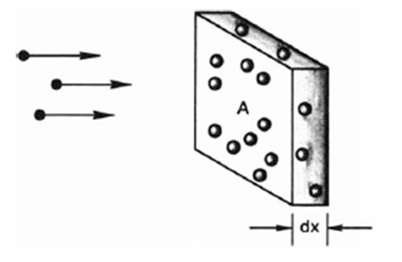
\includegraphics[width=0.6\linewidth]{fig5.2.png}
  \caption{断面積の定義の説明}
  \label{fig5.2}
\end{figure}

層の中の原子数は$n_nA\,dx$より，原子によって阻止される確率は，

\[
  \frac{n_nA\,dx\cdot \sigma}{A} = n_n\sigma\,dx
\]
もし電子束$\Gamma$がこの層に入射されたとすると，層に阻まれずに反対側に現れる電子束は

\[
  \Gamma' = \Gamma (1-n_n\sigma \,dx)
\]
となる．したがって，距離による$\Gamma$の変化は，


\begin{gather}
  d\Gamma/dx = -n_n\sigma \Gamma \notag \\
  \Gamma = \Gamma_0e^{-n_n\sigma x} \equiv \Gamma_0e^{-x/\lambda_m} \label{5.1}
\end{gather}
である．これより，距離$\lambda_m$で，電子束ははじめの値の$1/e$に減少する．この$\lambda_m$が衝突における平均自由行程である．

\begin{equation}
  \boxed{\lambda_m = 1/n_n\sigma} \label{5.2}
\end{equation}
この「はじめの値の$1/e$に減少する」長さで定義するのは，デバイ長のときと同様である．

速度$v$の粒子の衝突間の平均時間は
\[
  \tau = \lambda_m/v
\]
より，衝突の平均周波数は
\begin{equation}
  \tau^{-1} = v/\lambda_m = n_n\sigma v \label{5.3} 
\end{equation}
もし，Maxwell分布中のすべての速度$v$の粒子について平均すると，一般的にいわれている衝突周波数$\nu$は次式で表される：

\begin{equation}
  \nu = n_n\overline{\sigma v} \label{5.4}
\end{equation}


\subsubsection{拡散パラメータ} \label{section5.1.2}
衝突を含んだ流体の運動方程式は，どんな種類の粒子に対しても以下の式で表される：

\begin{equation}
  mn\frac{d\bm{v}}{dt} = mn\left[\frac{\partial \bm{v}}{\partial t} + (\bm{v}\cdot\nabla)\bm{v}\right] = \pm en\bm{E} - \nabla p -mn\nu\bm{v} \label{5.5}
\end{equation}
式\eqref{5.5}を使いやすくするためには，$\nu$を一定であると仮定するのがよい．ここで，$\partial \bm{v}/\partial t =0$である定常状態を考えてみよう．
$\bm{v}$が十分に小さい（あるいは$\nu$が十分に大きい）ならば，衝突するまでの間に空間変化を伴うような領域に流体要素はほとんど移動せず，対流項$d\bm{v}/dt$も無視できる．というのも，
粒子は十分加速して空間構造を横切る前に衝突するため，対流項は小さくなるからである．

よって，式\eqref{5.5}の左辺を0として，等温プラズマ（$\gamma=1$）に対して，

\begin{align}
  \bm{v} &= \frac{1}{mn\nu}(\pm en\bm{E} - KT\nabla n) \notag \\
         &= \pm \frac{e}{m\nu}\bm{E} - \frac{KT}{m\nu}\frac{\nabla n}{n} \label{5.6}
\end{align}
を得る．この2つの係数はそれぞれ、\textcolor{red}{易動度}，\textcolor{red}{拡散係数}と呼ばれる：

\begin{equation}
  \boxed{\mu \equiv |q|/m\nu}\hspace{1pc}\text{（易動度）} \label{5.7}
\end{equation}
\begin{equation}
  \boxed{D \equiv KT/m\nu}\hspace{1pc} \text{（拡散係数）} \label{5.8}
\end{equation}
これら2つの輸送係数$\mu$，$D$は，次のEinsteinの関係式で結び付けられる：

\begin{equation}
  \boxed{\mu = |q|D/KT} \label{5.9}
\end{equation}
これらの定義を用いて，j種の粒子束$\Gamma_j$は，

\begin{equation}
  \boxed{\Gamma_j = n\bm{v}_j = \pm \mu_jn\bm{E} - D_j\nabla n} \label{5.10}
\end{equation}
と書ける．拡散に関するFickの法則はこの特殊な場合で，上記において$\bm{E}=0$あるいは粒子が電荷をもたぬ場合，すなわち$\mu=0$の場合に起こる：

\begin{equation}
  \boxed{\Gamma = -D\nabla n}\hspace{1pc}\text{Fickの法則} \label{5.11}
\end{equation}
この方程式は，拡散がランダムウォーク過程であることを単に表現しているに過ぎない．
高密度領域から低密度領域への正味の流束が生じるのは，単に高密度領域でより多くの粒子が動く，という簡単な理由から起きる．
したがって，この流束は明らかに密度勾配に比例する．だが，プラズマにおいてはFickの法則が必ずしも成立しない．
系統だった運動（プラズマ波）の可能性により，プラズマは真にランダムとは言えない方法で拡散することがある．


\subsection{拡散によるプラズマの減少} \label{section5.2}
\subsubsection{両極性拡散} \label{section5.2.1}







\begin{thebibliography}{99}
\bibitem{a} Francis F. Chen, Introduction to Plasma Physics and Controlled Fusion, Springer; Softcover reprint of the original 3rd ed., 2019\par
\url{http://library.unisel.edu.my/equip-unisel/custom/ebook_catalog/2016BookIntroductionToPlasmaPhysicsAndcompressed.pdf}
\bibitem{b} 宮本健郎, プラズマ物理の基礎, 朝倉書店 , 2014\par
\url{https://op.lib.kobe-u.ac.jp/opac/opac_details/?reqCode=fromlist&lang=0&amode=11&bibid=2002133568&opkey=B175679900718865&start=1&totalnum=4&listnum=1&place=&list_disp=20&list_sort=0&cmode=0&chk_st=0&check=0000}
\bibitem{c} EMANの物理学\par
\url{https://eman-physics.net/electromag/plasma.html}
\end{thebibliography}


\end{document}